\documentclass[12pt]{article}

\usepackage{natbib,hyperref,graphicx}
\usepackage[separate-uncertainty=true,multi-part-units=single]{siunitx}

\usepackage[margin=1.5cm,twoside]{geometry}

\usepackage[para]{footmisc}


\usepackage[compact]{titlesec}
% \titlespacing{\section}{0pt}{2ex}{1ex}
% \titlespacing{\subsection}{0pt}{1ex}{0ex}
% \titlespacing{\subsubsection}{0pt}{0.5ex}{0ex}

\DeclareSIUnit{\arcsec}{''}
\DeclareSIUnit{\mag}{\text{mag}}

\usepackage[utf8]{inputenc}
\usepackage{newunicodechar}
%\usepackage{libertine}

\DeclareRobustCommand{\okina}{%
  \raisebox{\dimexpr\fontcharht\font`A-\height}{%
    \scalebox{0.8}{`}%
  }%
}
\newunicodechar{ʻ}{\okina}
\newcommand{\omuamua}{\okina Oumuamua }


\title{ASTR480 Progress Report}
\author{Brayden Leicester \\[1ex]
\small{Supervisors: Michele Bannister and Ryan Ridden-Harper}
}
\begin{document}
\maketitle

%*Aim / background summary

\section{Background}

%To get all asteriods in TESS. 
This project aims to find and characterise the light curves of all the asteroids seen by the Transiting Exoplanet Survey Satellite (TESS). 
    %Why TESS
TESS is a large area, high cadence imaging , space telescope  \citep{Ricker2014}. 
TESS is tasked with observing one piece of sky for \qty{27}{\day} at a time (a sector), delivering \qtyproduct{96 x 24}{\degree} full frame images (FFIs) at regular intervals. 
With the initial cadence for these full frame images set to \qty{30}{\minute}, the time resolution of TESS is unparalleled, with a Nyquist frequency of \qty{1}{\per\hour}, as the mission was extended the length of the FFIs has come down to \qty{10}{\minute} and then \qty{200}{\second}. 
This high time resolution and observation area does come at the cost of spatial resolution, as the pixels are each \qty{21}{\arcsec} square.
There have been attempts before to find and classify the asteroids in TESS data before by \citet{Pal2018, Pal2020}. This work aims to extend their study to more sectors, and to use a different data reduction method, the \texttt{TESSreduce} package \citep{Ridden-Harper2021}.
%TODO expand here...
Because of the survey properties, TESS provides a self-consistent way to measure the properties of asteroids over the full sky.   
Another beneficial part of this work is that as part of a full sky transient survey using TESS, \texttt{TESSELLATE} (Ridden-Harper and Roxburgh et al., in prep), asteroids are transient objects that spike the brightness of a pixel for only a few frames.
The goal of finding all the asteroids will allow for the removal of these spikes from the transient pipeline, as well as to understand the asteroid population better.  


    %Why Asteroids
Asteroids are a key class of solar system objects. 
Understanding their rotation properties has long been of interest to astronomers \citep[e.g.][]{Weidenschilling1981,Harris1994}. %Omuamu
High amplitude variation has come to the forefront of questions about asteroid properties because of the first interstellar object, 1I/\omuamua \citep[see][for a review]{Bannister2019}. 
\omuamua was measured to have a rotation period of \qty{8.67(0.34)}{\hour} \citep{Belton2018} and seemed to be tumbling \citep[e.g.][]{Drahus2018,Fraser2018}. 
The peak to peak amplitude variation of \qty{2.5}{\mag} \citep{Meech2017} of the double peaked light curve is of interest, as this is much higher than most asteroids, and it implies a large axis ratio. 
With the full sky survey of bright asteroids, we hope to find many asteroids with such a large amplitude variation, and to see just how rare \omuamua is.  

\section{Work So Far}
%* Method / Initial Results

%Querry and interpolate
To check for asteroids in the TESS data, the positions of the asteroids with time are required.
For most asteroids, their orbital elements are well known, so it is a matter of looking them up and cross-matching with transients in the TESS data.
Python was used to make API calls to {Skybot}\footnote{\href{https://vo.imcce.fr/webservices/skybot/}{Skybot: https://vo.imcce.fr/webservices/skybot/}} to get positions of asteroids in a cone search box in right ascension (RA) and  declination (Dec) space.
As TESS sectors are \qty{27}{\day} long, querying every \qty{12}{\hour} is manageable.
These positions are still very sparsely spaced in time compared to the TESS data, so an interpolation is needed to bridge the gap.
With TESS data coming in $\frac12\unit{\hour}$ chunks, 24 interpolated points are needed between each API call.
This interpolation should be accurate, as asteroids move at close to a TESS pixel per FFI on average \citep{Pal2018,Pal2020}, and checking against a higher frequency query to {JPL Horizons}\footnote{\href{https://ssd.jpl.nasa.gov/horizons/}{JPL Horizons: https://ssd.jpl.nasa.gov/horizons/}} confirmed this accuracy.
For the shorter FFIs, the asteriods will be move fewer pixels per frame, which could cause slight mismatches between the interpolation and the detections. 
Horizons was also used get properties of the individual asteroids, such as the absolute magnitude $H$. 
For the faster TESS data, more interpolated points are needed, but a smaller the change in position between each point.
These interpolated positions can be seen in \autoref{Fig:interpPos} for a cut from \texttt{TESSELLATE}. 
There are a few interesting features, such as the asteroids are moving in the same direction, indicated by the colouring, they come in from low RA and Dec and tend to increase both coordinates as the month of the sector progresses. 
There is also a large size range in this slice of sky, ranging over \qty{5}{\mag} in absolute magnitude, which can be seen in the alpha (or transparency) of the tracks in \autoref{Fig:interpPos}. 

%Match to detections
Matching these interpolated positions to \texttt{TESSELLATE} detections is important to lower the unknown transient outputs of this pipeline. 
Using the \texttt{KDTree} algorithm \citep{Maneewongvatana1999} as implemented in \texttt{SciPy} \citep{2020SciPy-NMeth}, the RA and Dec coordinates of the interpolated points and the detections can be compared and matched together. 
Filtering this \texttt{KDTree} output by restricting the time between spatially coincident matches to less than \qty{0.1}{\day} stops any accidental matches in position from non-asteroid detections. 
    
%light curves; detected VS forced interpolated 
There are two sets of points to take light curves from. 
The matches from the detections, which already have a flux calculated, and the interpolated points themselves, which are more numerous but require forcing the photometry. 
There were some challenges getting the flux of the interpolated points, even when \texttt{TESSELLATE} has already reduced all the FFIs of interest, due to the timing of the TESS frames, but these were identified and corrected for.
Not every interpolated point gets a match, due to a variety of reasons, %pass in front of stars, dip below limiting mag, bad pipeline, not extreme enough of a difference between frames 
so a comparison between the two light curves is interesting. 
\autoref{Fig:DifFlux} shows these two light curves for a chosen asteroid, ``Ruff''. 
This was picked as it has a high number of points matched to detections.
% There are more interpolated points than matched points, as not ever interpolated point gets matched to a detection.
There seems to be a systematic offset between the fluxes, with the interpolated points having consistently lower flux, (here the means differ by 58 counts)
Adjusting aperture to sum the fluxes over to the ``centre of mass'' of the asteroid in each frame does not alleviate this problem. 

\section{Future Work}
%* Future work

%Periods and amplitueds for everything detected
The next part of my analysis has to do with determining the periods and amplitudes of each asteroid's light curve.
For this there are a few methods I can try; using the \texttt{Lightkurve} \citep{Lightkurve2018} package built for period analysis of TESS (and Kepler) data of variable stars or peel back a layer of abstraction and use the Lomb-Scargle periodogram as implemented by \texttt{Astropy}\cite{Astropy2022}. 
Some trialling of both methods is needed, as preliminary testing reveals of interesting similarities and differences between the packages. 
There will be differences in the period between the matched points and the interpolated points, not just because of the difference in average flux, but also from the larger number of points. This difference needs to be carefully thought through to understand what is the more likely period.


%Run on server
The \texttt{TESSELLATE} pipeline has been running on the OzSTAR supercomputing facilities. 
After I am confident that all the parts of the asteroid detection and subsequent light curve analysis works as required, the same code can be refactored to work on OzSTAR and a large-scale analysis of all the processed TESS sectors can be run. 
Only after this has completed can the asteroid population statistics can be computed. 
I will be looking for completeness of detections of asteroids, as well as accuracy of periods and amplitude variation.


% \section{Figures}
%*Figures:
\newgeometry{twocolumn,margin=1.5cm,twoside}

\begin{figure}
  \centering
    \includegraphics[width =\columnwidth]{../Test Code/Testing Figures/interpPos\_22\_2\_3\_4.pdf}
    \caption{The interpolated positions of asteroids in one cut of a TESS sector. 
    The colours of the lines are time sequenced, as shown in the colour bar.
    The alpha of the colours are scaled by the absolute magnitude $H$ of the asteroid, queried from JPL Horizons. 
    Both celestial (RA and Dec) coordinates and ecliptic (ecLon and ecLat) coordinates axes are shown.
    }
    \label{Fig:interpPos}
\end{figure}



\begin{figure}
  \centering
  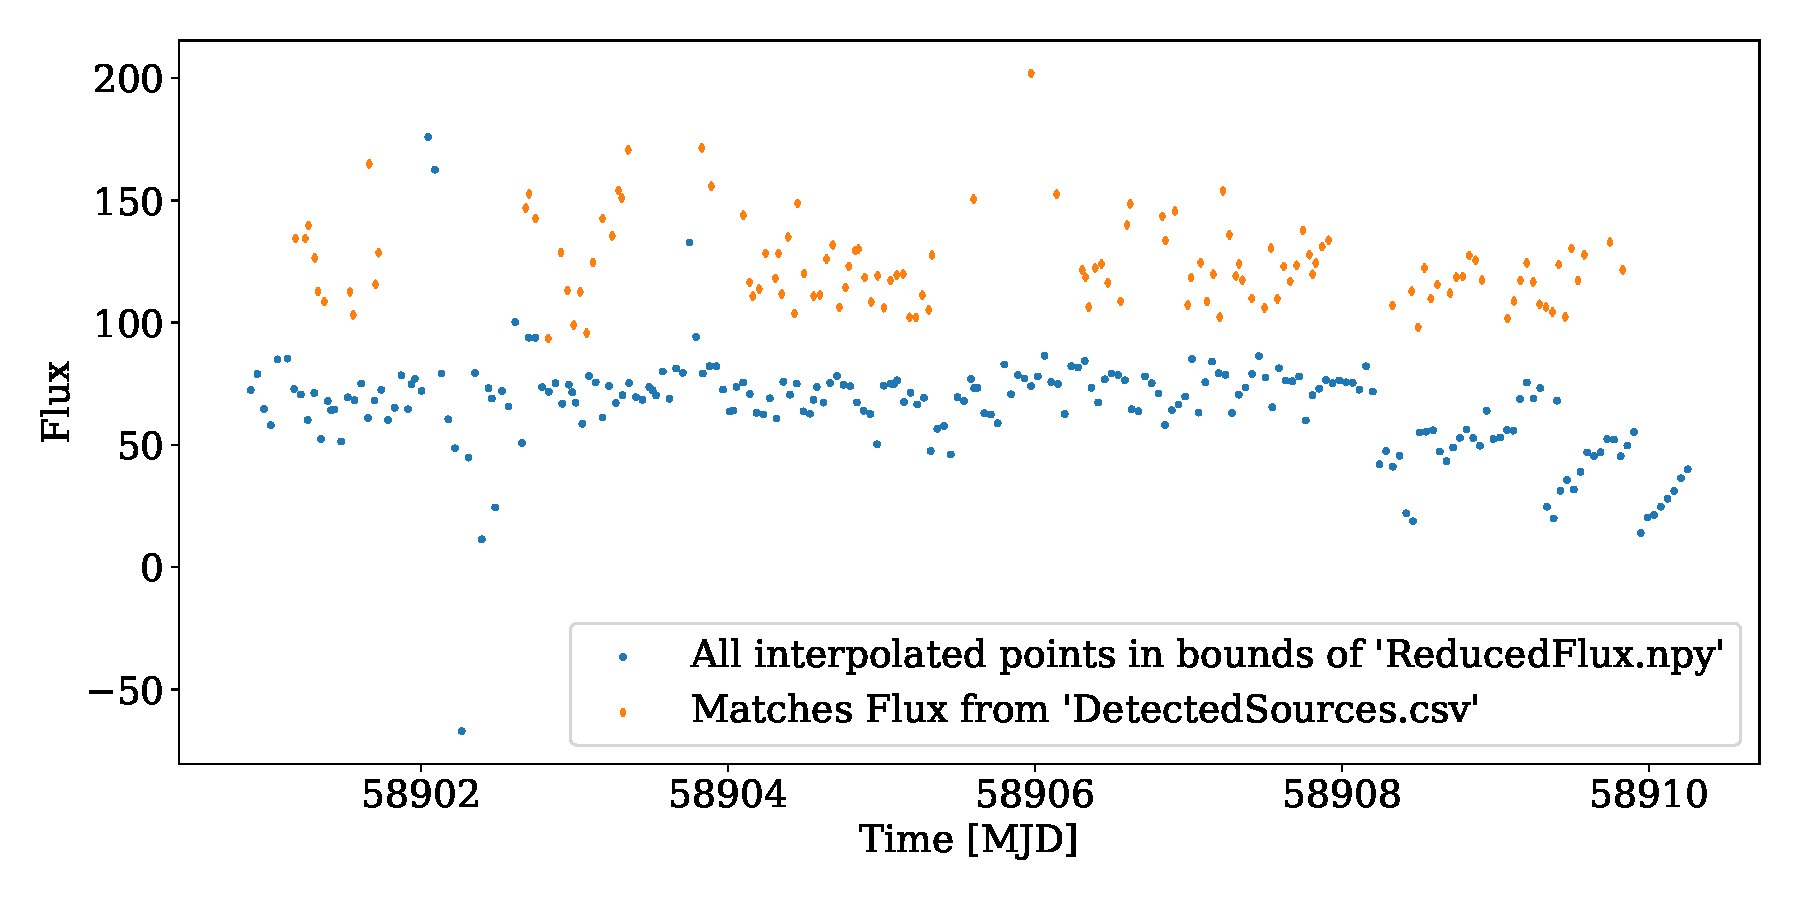
\includegraphics[width =\columnwidth]{../Test Code/Testing Figures/differentFluxes Ruff .pdf}
  \caption{The light curves of the asteroid ``Ruff'', with the flux of the interpolated positions in blue circles and the flux from the matches to detected sources in orange diamonds.
  The Flux axis is measured in counts, as calculated by \texttt{TESSreduce}, and the times are in Modified Julian Date.}
  \label{Fig:DifFlux}
\end{figure}
    

% \section{Acknowledgements}
% %OzSTAR asks for:
% \small
% This work was performed on the OzSTAR national facility at Swinburne University of Technology. 
% The OzSTAR program receives funding in part from the Astronomy National Collaborative Research Infrastructure Strategy (NCRIS) allocation provided by the Australian Government, and from the Victorian Higher Education State Investment Fund (VHESIF) provided by the Victorian Government.


%H-scaled pos plot of higher cam/less asteroids. 
%Both light curves (interp and detect)
%? another one?


%*Bib
% \newgeometry{twocolumn,margin=1.5cm, left=3cm}
% \newpage
\def\bibfont{\tiny}
\bibliographystyle{jphysicsB}
\bibliography{../Notes/bibfile.bib}
\end{document}



